\section{Resultados}
%Deben incluir los resultados de los experimentos, utilizando el formato más adecuado
%para su presentación. Deberón especificar claramente a qué experiencia corresponde
%cada resultado. No se incluirán aquí corridas de máquina. Algo fundamental en su
%aprendizaje en la materia es la presentación de resultados de forma clara y concisa para
%el lector.



\subsection{Experimento 1}
Se procedió a ejecutar el método de kNN variando k, para K = 2, 10 y 20 con k $\in$ $\{$2, 30, 100, 500$\}$ .

Se observo que la memoria utilizada por el programa era de 127,6 Mb en sus faces iniciales, hasta que en un punto se queda en 380,5 Mb.

Los resultados obtenidos fueron los siguientes:
\begin{itemize}
\item Con K = 2\\
\end{itemize}

\begin{table}[H]
\centering
\begin{tabular}{|r|r|r|}
\hline
\multicolumn{1}{|c|}{k} & \multicolumn{1}{c|}{Tiempo} & \multicolumn{1}{c|}{Tasa} \\ \hline
2 & 3297,38 & 0,952476 \\ \hline
30 & 3307,48 & 0,942452 \\ \hline
100 & 3344,49 & 0,91681 \\ \hline
500 & 3760,26 & 0,844905 \\ \hline
\end{tabular}
\caption{Tasas para Knn variando k para dos particiones}
\label{}
\end{table}

\bigskip
\bigskip
\bigskip

    \begin{figure}[H]
    \centering
    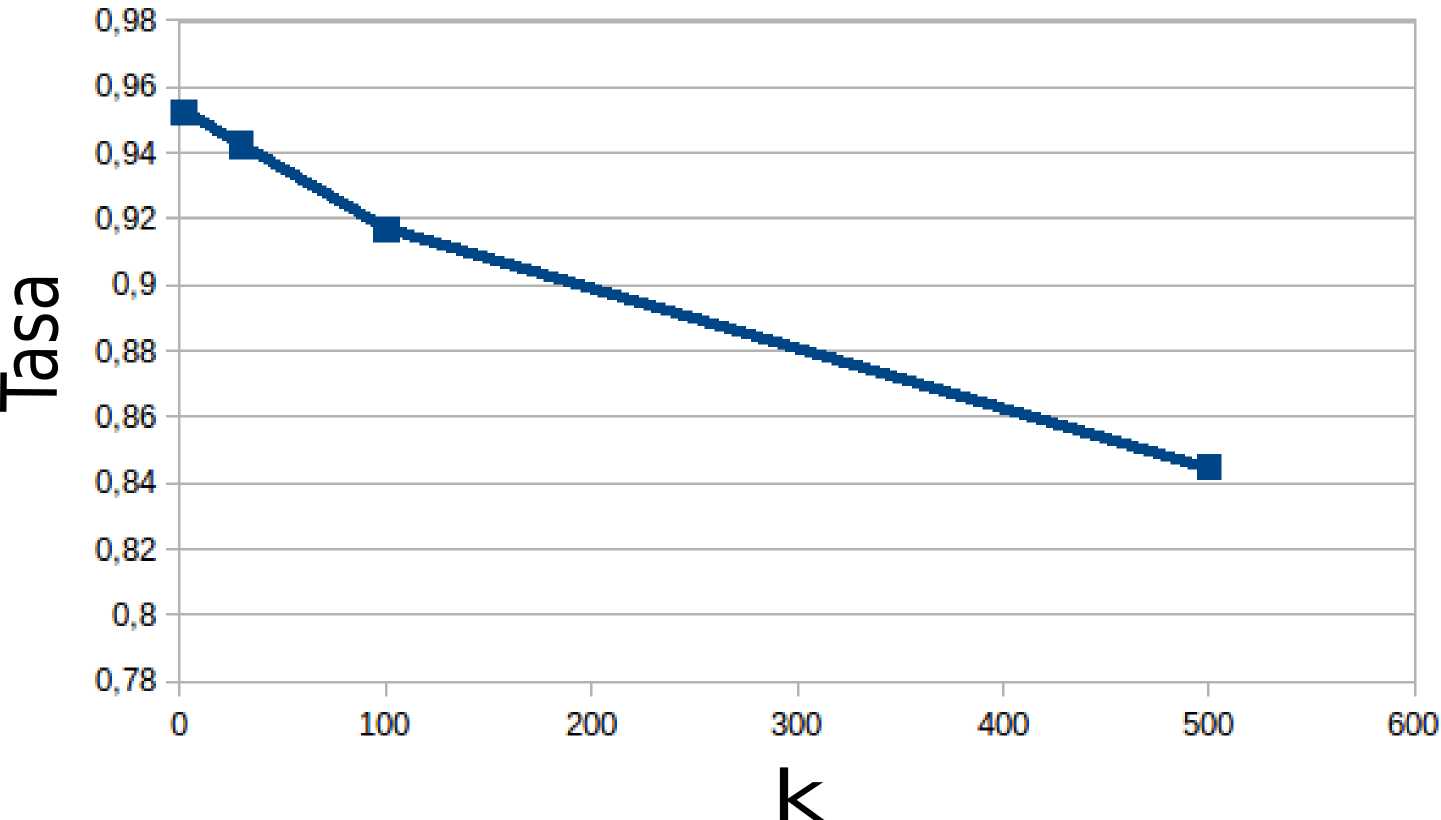
\includegraphics[scale=0.3]{Graficos/knnTasa2.png}
    \caption{Tasas para Knn variando k para dos particiones}
	\label{knnTasa2}
    \end{figure}
\bigskip
\bigskip
\bigskip






\begin{itemize}
\item Con K=10\\
\end{itemize}

\begin{center}

\begin{table}[H]
\centering
\begin{tabular}{|r|r|r|}
\hline
%\multicolumn{ 3}{|c|}{kNN variando k con K = 10} \\ \hline
\multicolumn{1}{|c|}{k} & \multicolumn{1}{c|}{Tiempo} & \multicolumn{1}{c|}{Tasa} \\ \hline
2 & 5853,64 & 0,96169 \\ \hline
30 & 5881,12 & 0,952262 \\ \hline
100 & 6026,68 & 0,93169 \\ \hline
500 & 6845,26 & 0,878833 \\ \hline
\end{tabular}
\caption{Resultados para Knn variando k para diez particiones}
\label{}
\end{table}
\end{center}

\bigskip
\bigskip
\bigskip

    \begin{figure}[H]
    \centering
    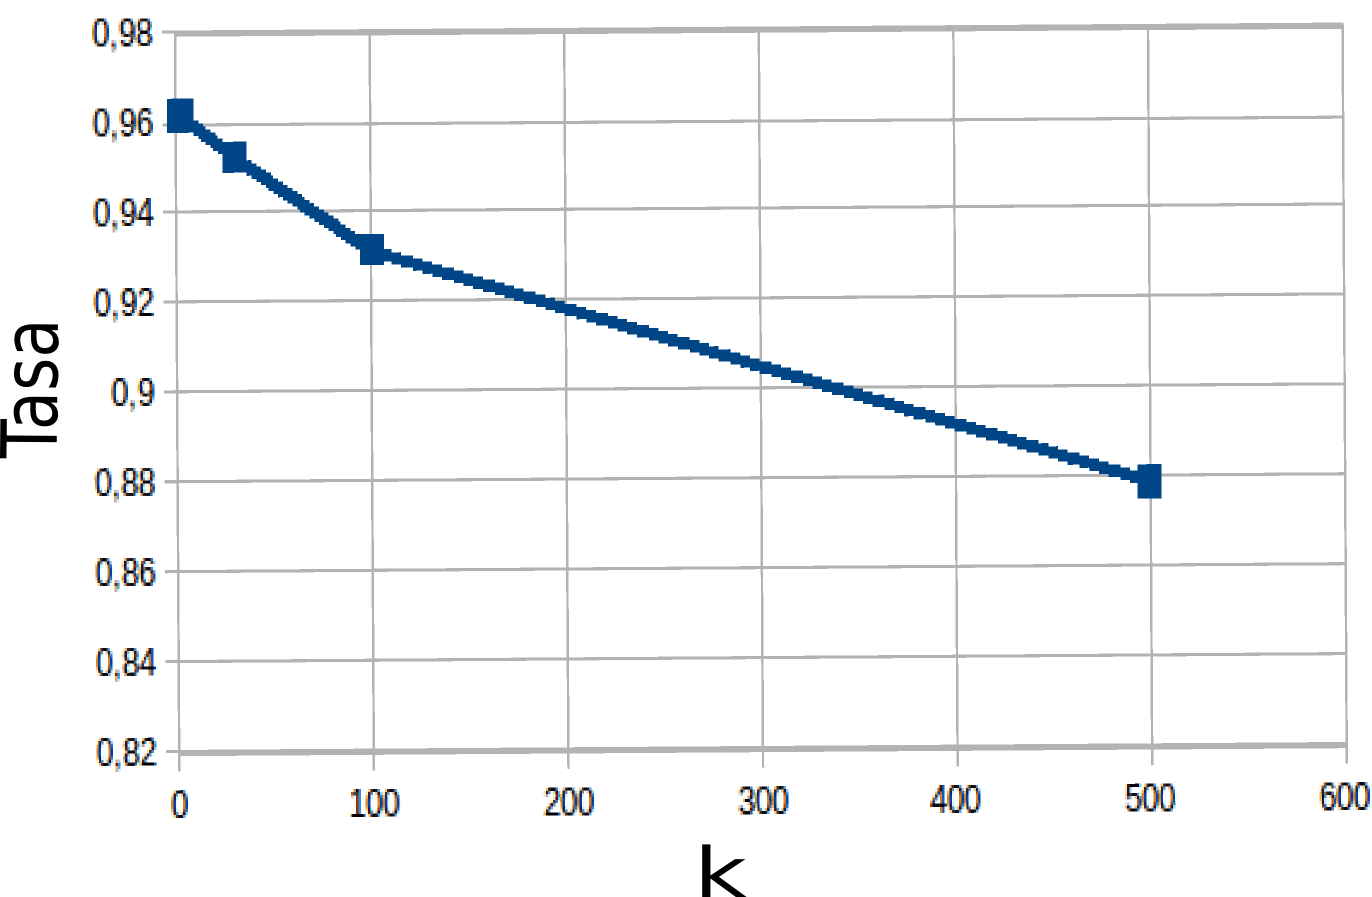
\includegraphics[scale=0.3]{Graficos/knnTasa10.png}
    \caption{Tasas para Knn variando k para diez particiones}
	\label{knnTasa10}
    \end{figure}
\bigskip
\bigskip
\bigskip




\begin{itemize}
\item Con K = 20\\
\end{itemize} 

\begin{table}[H]
\centering
\begin{tabular}{|r|r|r|}
\hline
\multicolumn{1}{|c|}{k} & \multicolumn{1}{c|}{Tiempo} & \multicolumn{1}{c|}{Tasa} \\ \hline
2 & 44812,6 & 0,962381 \\ \hline
30 & 44730,7 & 0,953167 \\ \hline
100 & 26247 & 0,933429 \\ \hline
500 & 5752,72 & 0,881381 \\ \hline
\end{tabular}
 \caption{Tasas para Knn variando k para veinte particiones}
\label{}
\end{table}
\bigskip
\bigskip
\bigskip

    \begin{figure}[H]
    \centering
    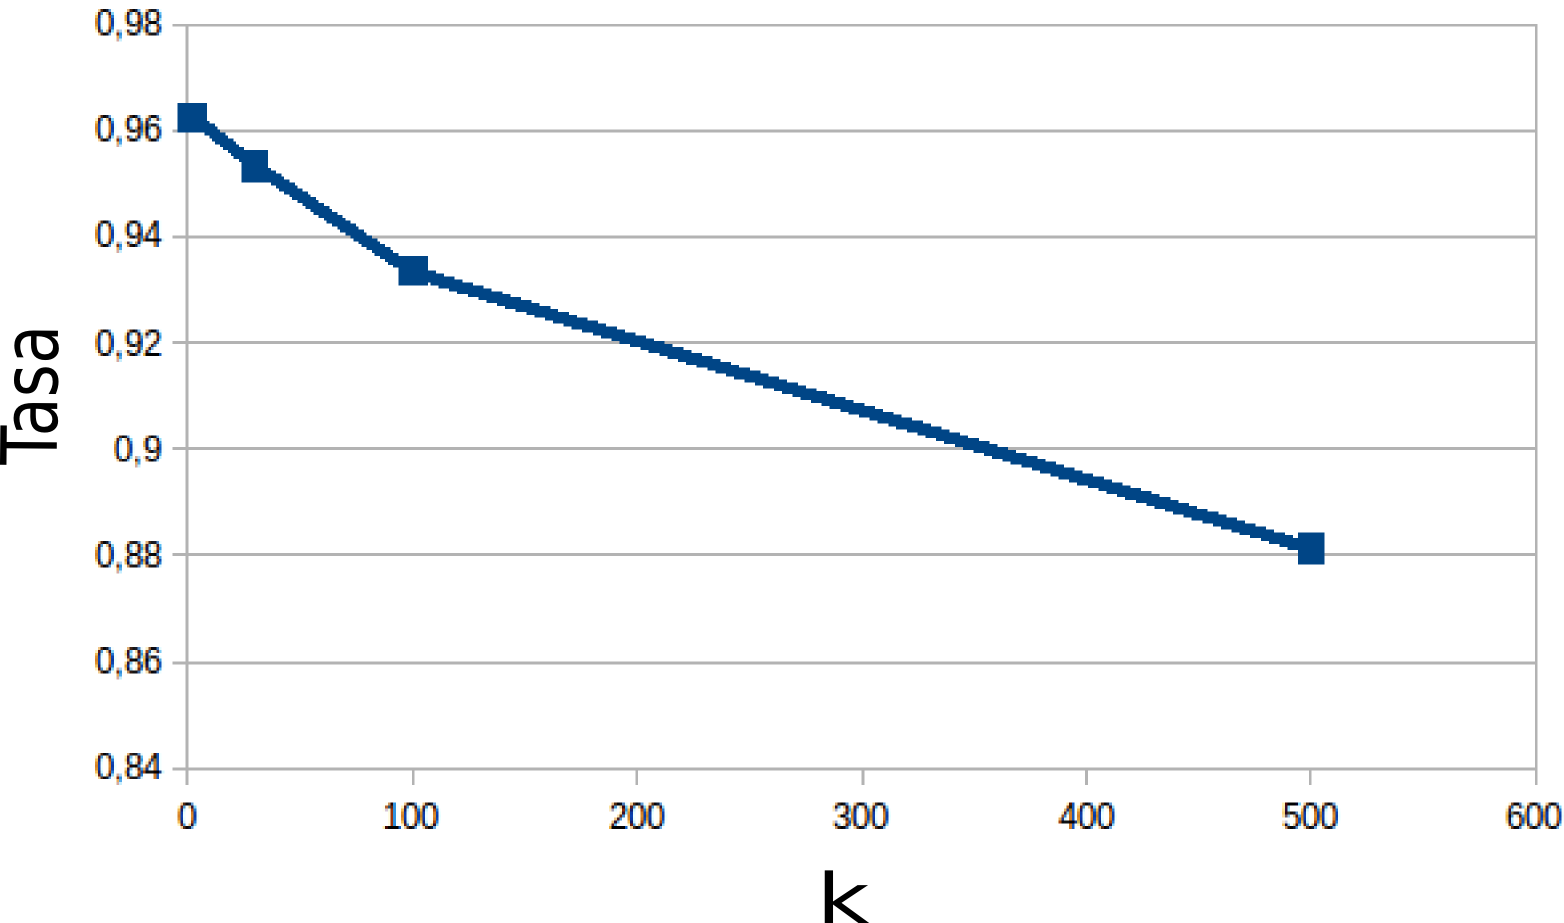
\includegraphics[scale=0.3]{Graficos/knnTasa20.png}
    \caption{Tasas para Knn variando k para veinte particiones}
	\label{knnTasa20}
    \end{figure}
\bigskip
\bigskip




Podemos ver que en ningún caso se obtiene una tasa del 100$ \% $. Con un k chico se corre el riesgo de que los vecinos mas cercanos no sean los correctos por una situación especial que pueda llegar a ocurrir, y entonces el dígito no sea reconocido. Sin embargo se comprueba empíricamente que con un k grande las tasas disminuyen apreciablemente. Esto se lo podemos atribuir a que hay una probabilidad no despreciable de que un dígito a reconocer este mas cercano a un dígito distinto que a uno igual. No es una cuestión de falta de dígitos iguales al que se esta reconociendo. Por ejemplo al tomar 500 vecinos mas cercanos, no es que no halla sido posible tomar a estos 500 como el dígito a reconocer por falta de este ultimo en la matriz de train, sino que en lugar de tomarse un dígito igual, se toma uno distinto, pero mas cercano.

También podemos ver que al incrementar k se obtiene un tiempo mayor. Esto se debe a que en el algoritmo de knn se debe en cada paso, recorrer un vector de tamaño k donde se encuentran los mas cercanos, ir actualizandolo. 


\subsection{Experimento 2}
Se procedió a ejecutar el método de kNN+PCA variando $\alpha$, para K = 2, 10 y 20 con k = 2.\\ 
Los resultados obtenidos fueron los siguientes:
\begin{itemize}
\item Con K = 2\\

    
\item Con K = 10\\

\item Con K = 20\\
\end{itemize}


